\documentclass{article}

\usepackage{fullpage, graphicx, verbatim, float, subcaption,caption}
\title{Output From Maximum Depth Simulations}
\begin{document}
\maketitle

\section{Boxplots of Estimated Dimensional Probabilities}


\begin{figure}[H]
        \centering
        \begin{subfigure}[b]{0.3\textwidth}
                \centering
                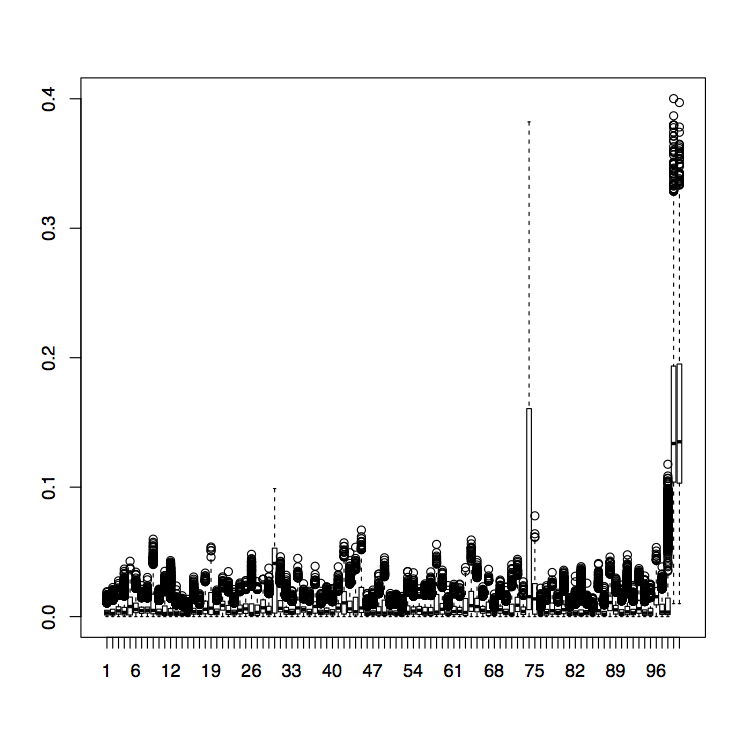
\includegraphics[width=\textwidth]{c1_boxp}
                \caption{Max Depth 1}
                \label{fig:gull}
        \end{subfigure}%
        ~ %add desired spacing between images, e. g. ~, \quad, \qquad etc. 
          %(or a blank line to force the subfigure onto a new line)
        \begin{subfigure}[b]{0.3\textwidth}
                \centering
                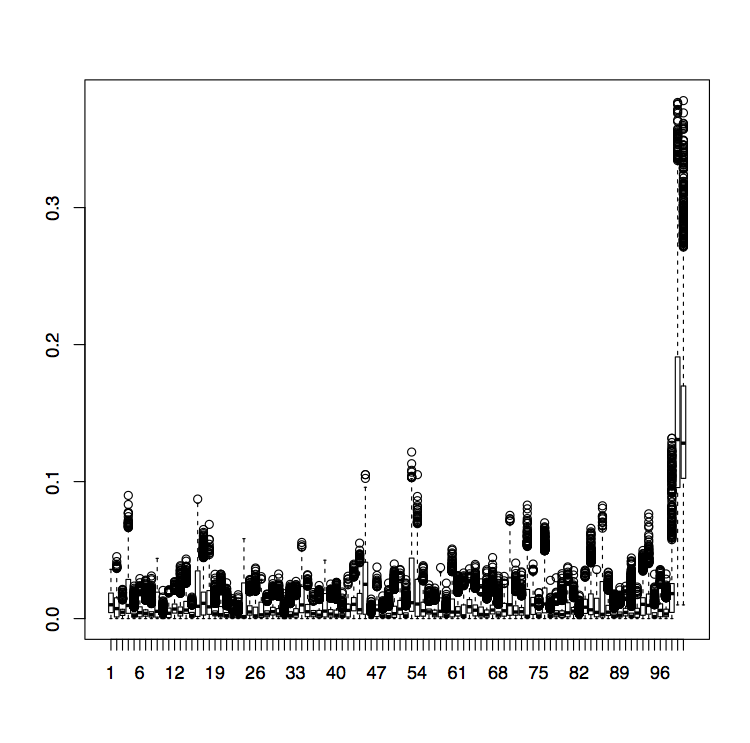
\includegraphics[width=\textwidth]{c2_boxp}
                \caption{Max Depth 2}
                \label{fig:tiger}
        \end{subfigure}
        ~ %add desired spacing between images, e. g. ~, \quad, \qquad etc. 
          %(or a blank line to force the subfigure onto a new line)
        \begin{subfigure}[b]{0.3\textwidth}
                \centering
                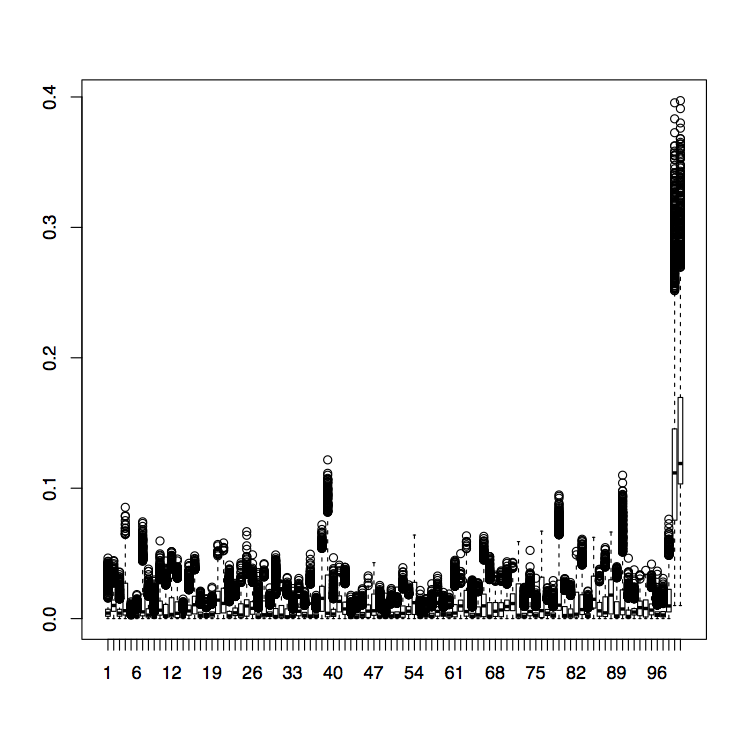
\includegraphics[width=\textwidth]{c3_boxp}
                \caption{Max Depth 3}
                \label{fig:mouse}
        \end{subfigure}
        \caption{Pictures of Boxplots for Maximum depths 1,2,3}\label{fig:Boxplots123}
\end{figure}


\begin{figure}[H]
        \centering
        \begin{subfigure}[b]{0.3\textwidth}
                \centering
                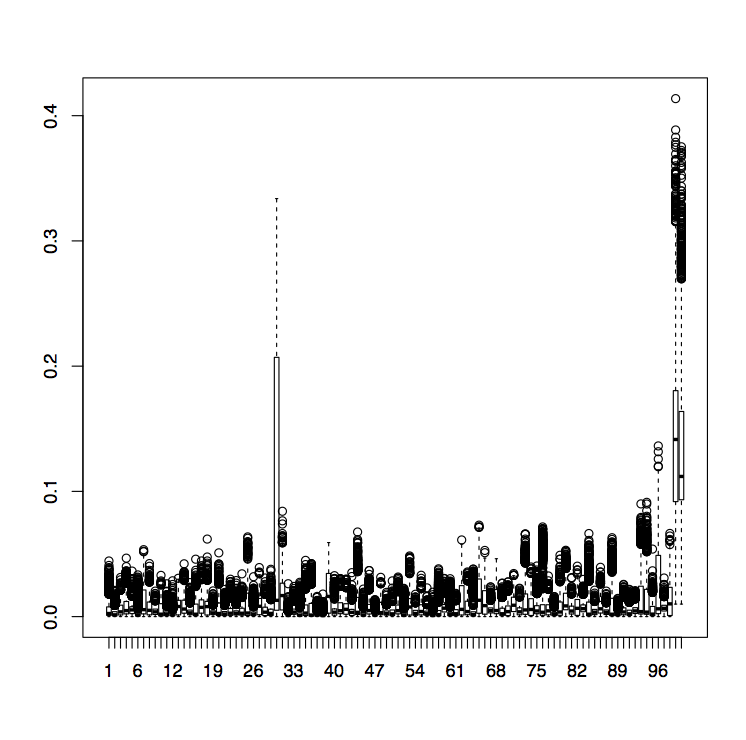
\includegraphics[width=\textwidth]{c4_boxp}
                \caption{Max Depth 4}
                \label{fig:gull}
        \end{subfigure}%
        ~ %add desired spacing between images, e. g. ~, \quad, \qquad etc. 
          %(or a blank line to force the subfigure onto a new line)
        \begin{subfigure}[b]{0.3\textwidth}
                \centering
                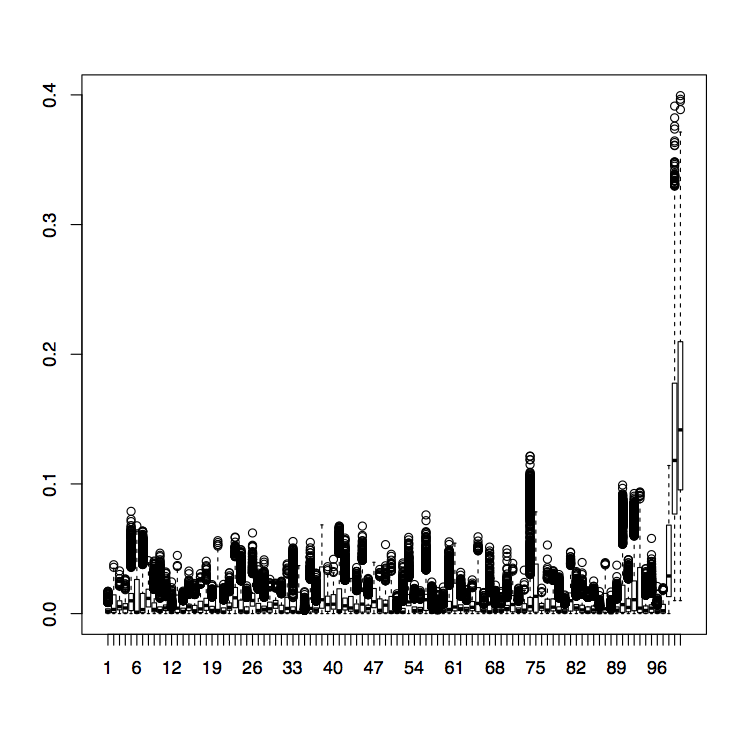
\includegraphics[width=\textwidth]{c5_boxp}
                \caption{Max Depth 5}
                \label{fig:tiger}
        \end{subfigure}
        ~ %add desired spacing between images, e. g. ~, \quad, \qquad etc. 
          %(or a blank line to force the subfigure onto a new line)
        \begin{subfigure}[b]{0.3\textwidth}
                \centering
                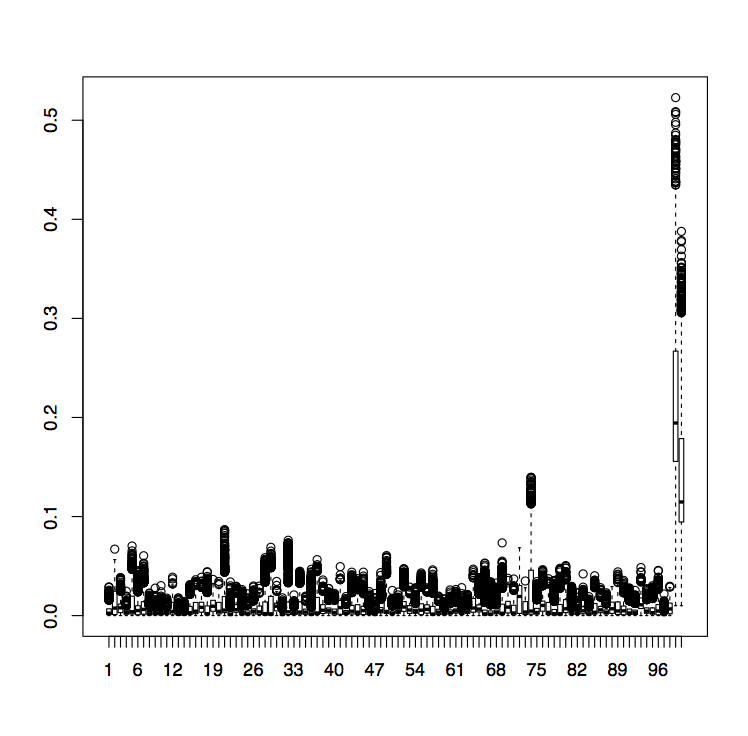
\includegraphics[width=\textwidth]{c6_boxp}
                \caption{Max Depth 6}
                \label{fig:mouse}
        \end{subfigure}
        \caption{Pictures of Boxplots for Maximum depths 4,5,6}\label{fig:Boxplots456 }
\end{figure}

\begin{figure}[H]
        \centering
        \begin{subfigure}[b]{0.3\textwidth}
                \centering
                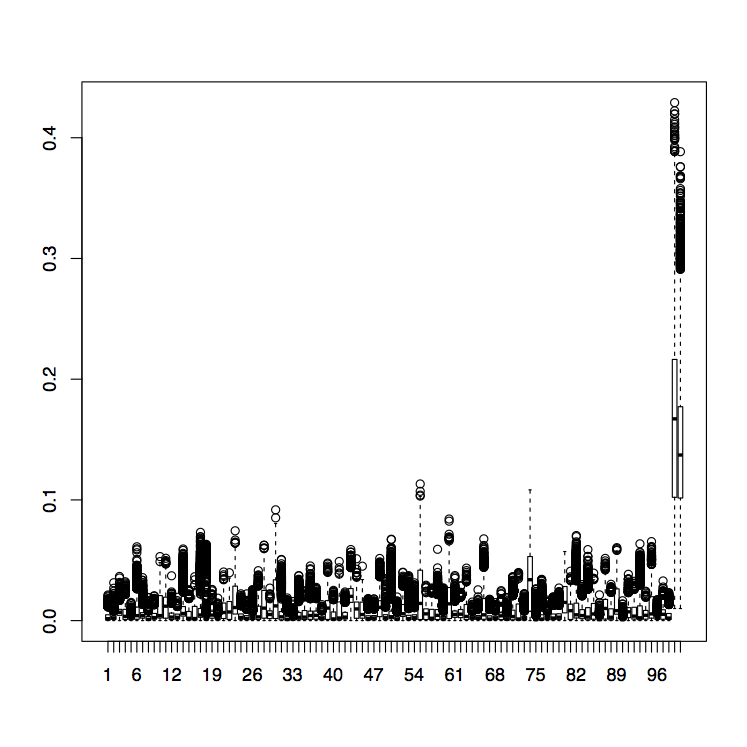
\includegraphics[width=\textwidth]{c7_boxp}
                \caption{Max Depth 7}
                \label{fig:gull}
        \end{subfigure}%
        ~ %add desired spacing between images, e. g. ~, \quad, \qquad etc. 
          %(or a blank line to force the subfigure onto a new line)
        \begin{subfigure}[b]{0.3\textwidth}
                \centering
                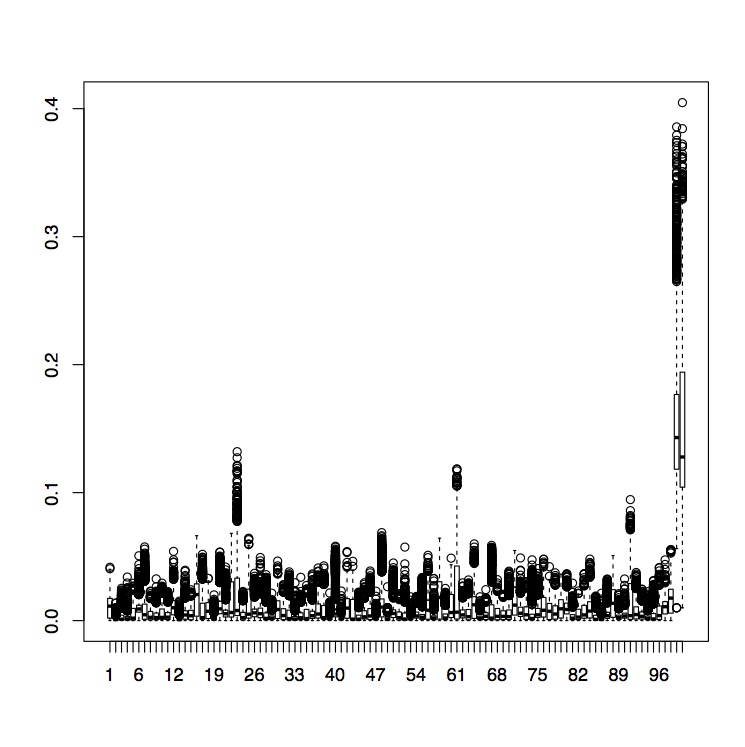
\includegraphics[width=\textwidth]{c8_boxp}
                \caption{Max Depth 8}
                \label{fig:tiger}
        \end{subfigure}
        ~ %add desired spacing between images, e. g. ~, \quad, \qquad etc. 
          %(or a blank line to force the subfigure onto a new line)
        \begin{subfigure}[b]{0.3\textwidth}
                \centering
                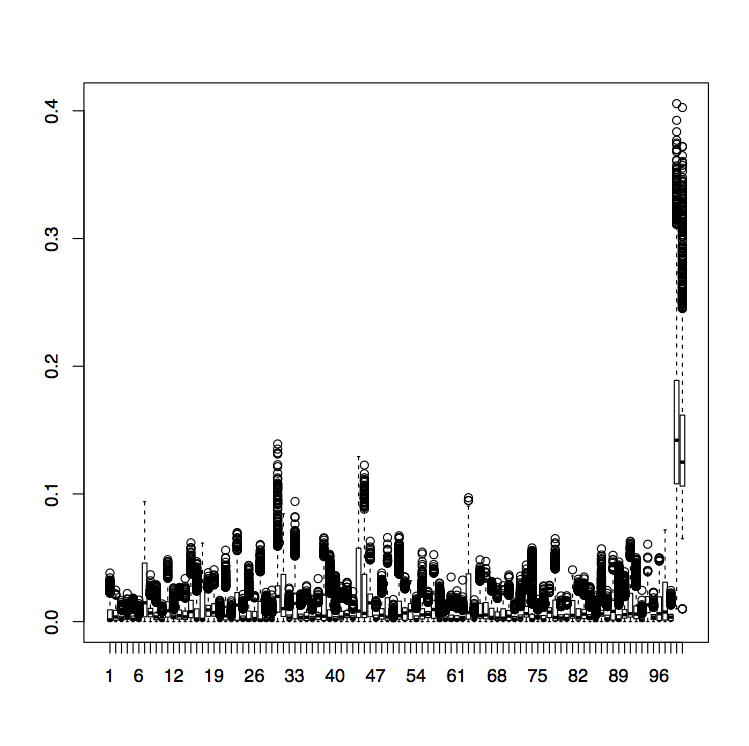
\includegraphics[width=\textwidth]{c10_boxp}
                \caption{Max Depth 10}
                \label{fig:mouse}
        \end{subfigure}
        \caption{Pictures of Boxplots for Maximum depths 7,8,10}\label{fig:Boxplots78_10 }
\end{figure}


\section{Depth Trace plots}

\begin{figure}[H]
        \centering
        \begin{subfigure}[b]{0.3\textwidth}
                \centering
                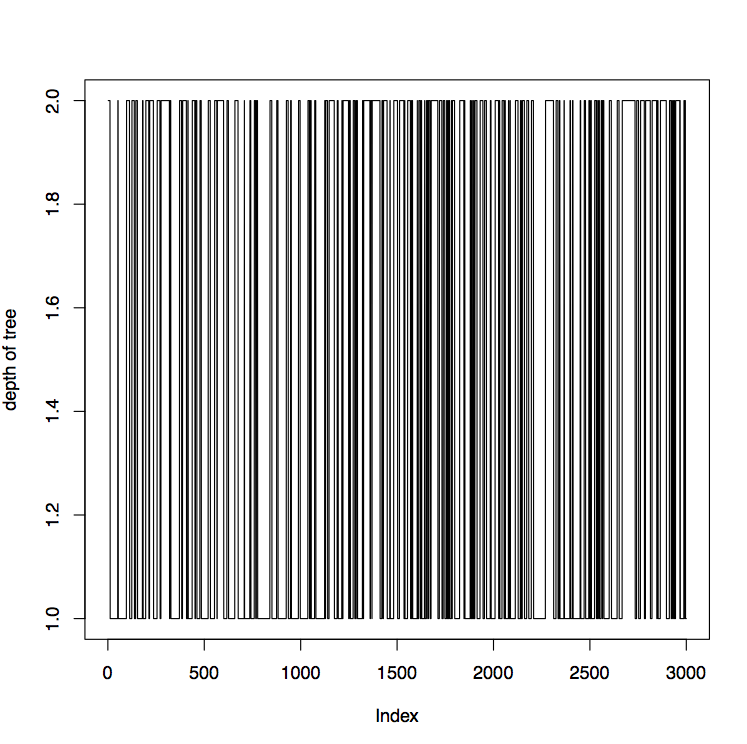
\includegraphics[width=\textwidth]{depth_c2}
                \caption{Max Depth 2}
                \label{fig:gull}
        \end{subfigure}%
        ~ %add desired spacing between images, e. g. ~, \quad, \qquad etc. 
          %(or a blank line to force the subfigure onto a new line)
        \begin{subfigure}[b]{0.3\textwidth}
                \centering
                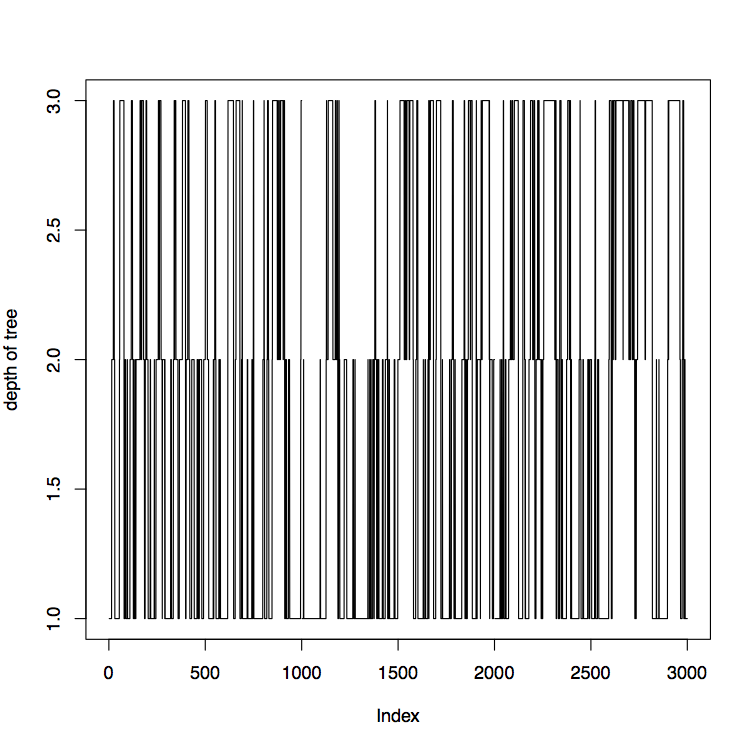
\includegraphics[width=\textwidth]{depth_c3}
                \caption{Max Depth 3}
                \label{fig:tiger}
        \end{subfigure}
        ~ %add desired spacing between images, e. g. ~, \quad, \qquad etc. 
          %(or a blank line to force the subfigure onto a new line)
        \begin{subfigure}[b]{0.3\textwidth}
                \centering
                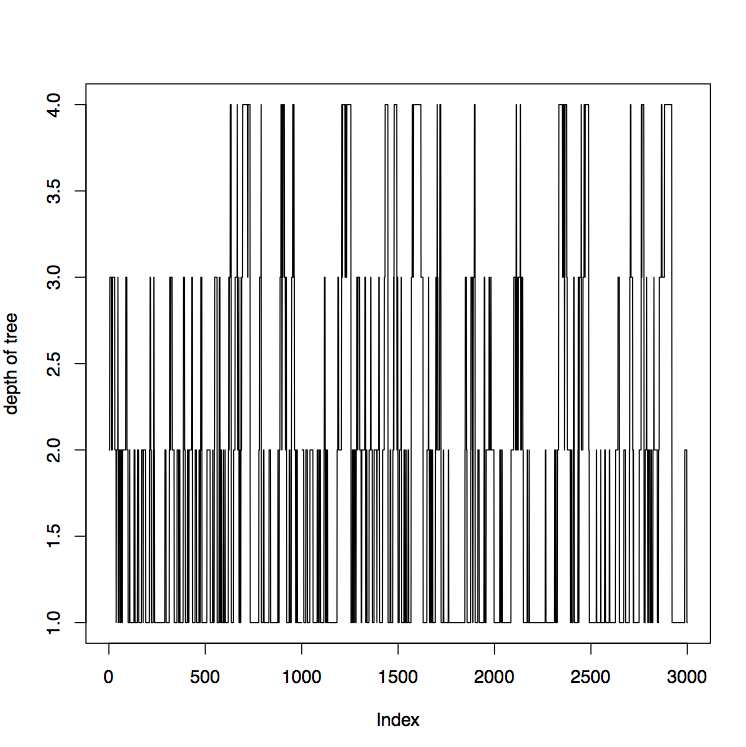
\includegraphics[width=\textwidth]{depth_c4}
                \caption{Max Depth 4}
                \label{fig:mouse}
        \end{subfigure}
        \caption{Traceplot of Depths for Maximum depths 2,3,4}\label{fig:Boxplots234}
\end{figure}


\begin{figure}[H]
        \centering
        \begin{subfigure}[b]{0.3\textwidth}
                \centering
                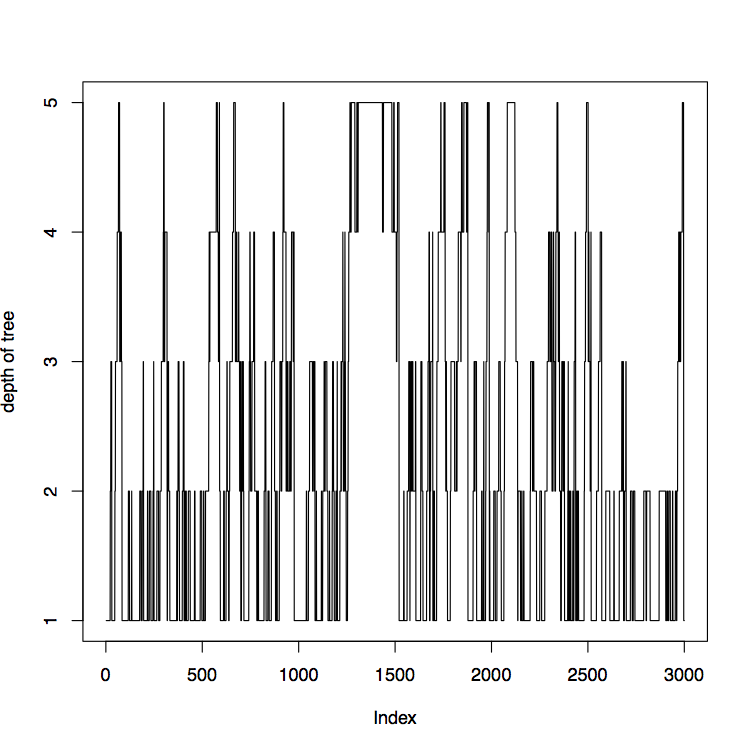
\includegraphics[width=\textwidth]{depth_c5}
                \caption{Max Depth 5}
                \label{fig:gull}
        \end{subfigure}%
        ~ %add desired spacing between images, e. g. ~, \quad, \qquad etc. 
          %(or a blank line to force the subfigure onto a new line)
        \begin{subfigure}[b]{0.3\textwidth}
                \centering
                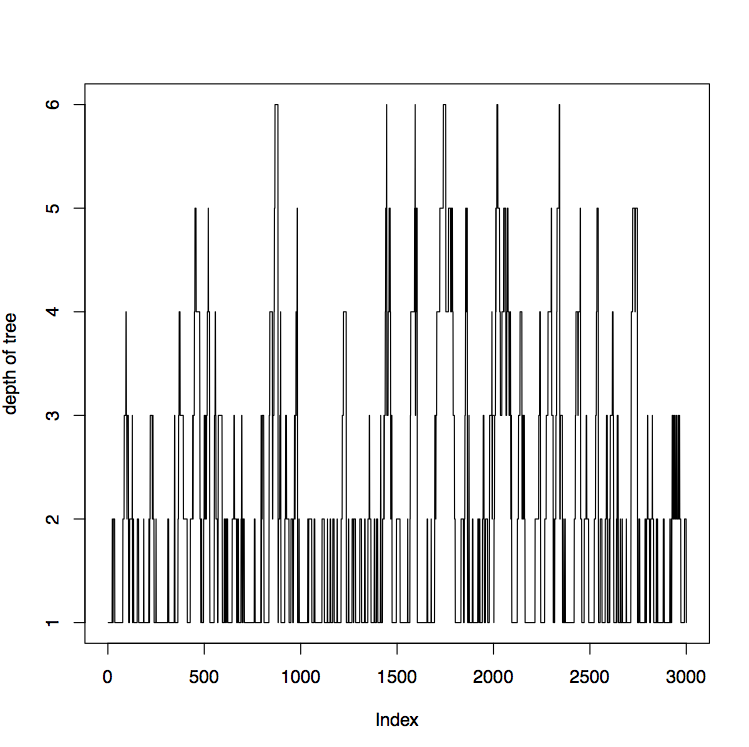
\includegraphics[width=\textwidth]{depth_c6}
                \caption{Max Depth 6}
                \label{fig:tiger}
        \end{subfigure}
        ~ %add desired spacing between images, e. g. ~, \quad, \qquad etc. 
          %(or a blank line to force the subfigure onto a new line)
        \begin{subfigure}[b]{0.3\textwidth}
                \centering
                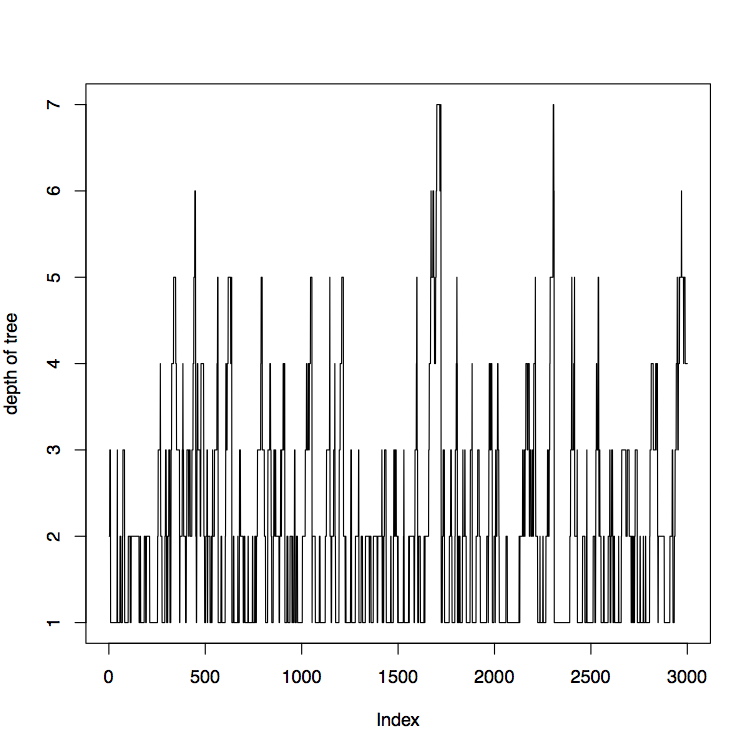
\includegraphics[width=\textwidth]{depth_c7}
                \caption{Max Depth 7}
                \label{fig:mouse}
        \end{subfigure}
        \caption{Traceplot of Depths for Maximum depths 5,6,7}\label{fig:Boxplots567 }
\end{figure}

\begin{figure}[H]
        \centering
        \begin{subfigure}[b]{0.3\textwidth}
                \centering
                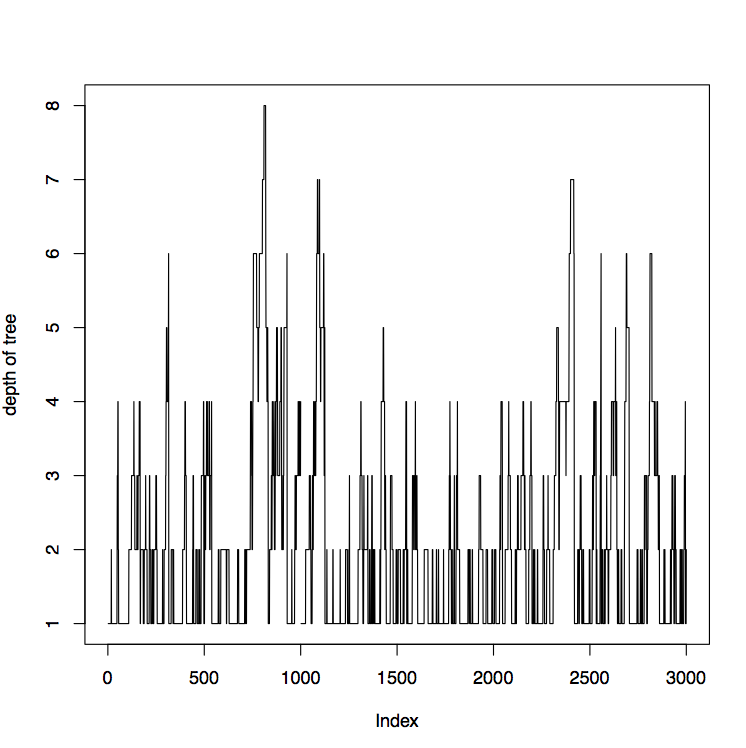
\includegraphics[width=\textwidth]{depth_c8}
                \caption{Max Depth 8}
                \label{fig:gull}
        \end{subfigure}%
        ~ %add desired spacing between images, e. g. ~, \quad, \qquad etc. 
          %(or a blank line to force the subfigure onto a new line)
        \begin{subfigure}[b]{0.3\textwidth}
                \centering
                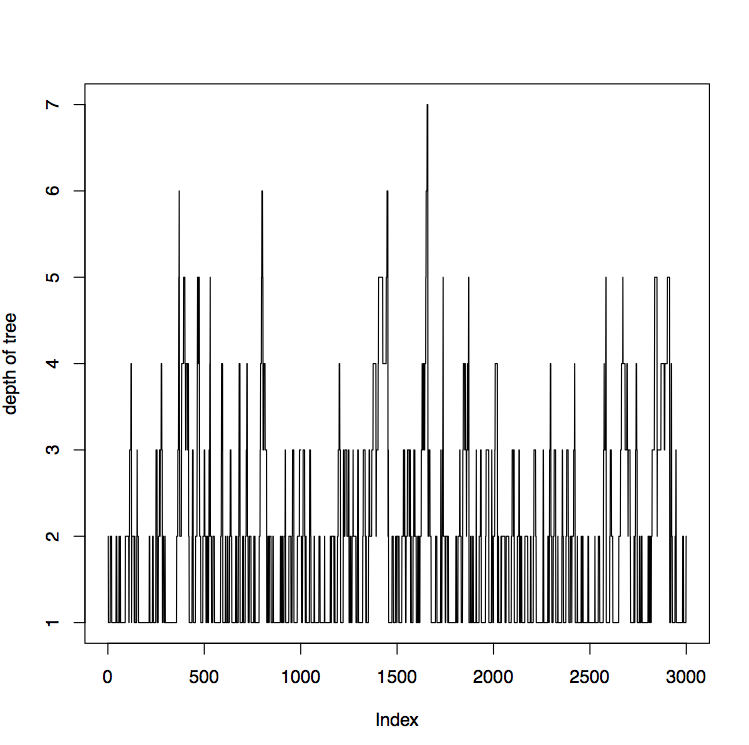
\includegraphics[width=\textwidth]{depth_c9}
                \caption{Max Depth 9}
                \label{fig:tiger}
        \end{subfigure}
        ~ %add desired spacing between images, e. g. ~, \quad, \qquad etc. 
          %(or a blank line to force the subfigure onto a new line)
        \begin{subfigure}[b]{0.3\textwidth}
                \centering
                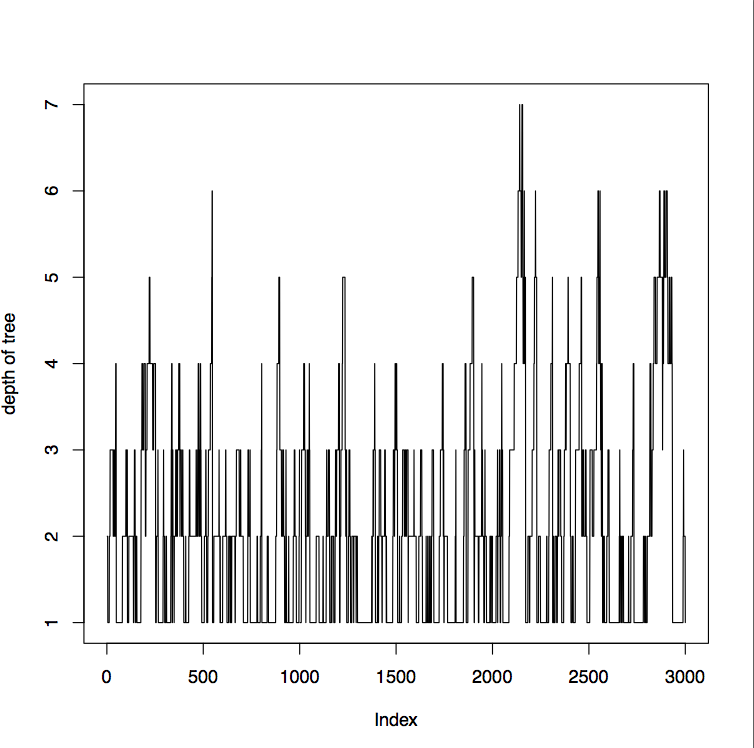
\includegraphics[width=\textwidth]{depth_c10}
                \caption{Max Depth 10}
                \label{fig:mouse}
        \end{subfigure}
        \caption{Traceplot of Depths for Maximum depths 8,9,10}\label{fig:Boxplots78_10}
\end{figure}


\end{document}